\section{Hasil agregat perdagangan Indonesia}\label{sec:aggregate}
\subsection{Dukungan level belum kuat pada model utama}
Agregat menggabungkan ekspor dan impor Indonesia dengan seluruh negara. Kedua model utama menggunakan 61 kuartal pada 2011Q1--2026Q1. ARDL memilih lag level $(2,3,0,4)$ untuk outcome, GDP Indonesia, aktivitas luar negeri dan kurs. NARDL memilih $(2,0,3,0,4)$, dengan dua posisi terakhir untuk partial sums positif dan negatif. Perbedaan lag ini merupakan hasil AIC pada himpunan kandidat, bukan bukti bahwa lag tersebut pasti menggambarkan proses ekonomi sebenarnya.

\begin{table}[!htbp]\centering
\caption{Bounds dan joint-X untuk agregat Indonesia}
{\small\setlength{\tabcolsep}{3pt}\renewcommand{\arraystretch}{1.15}
\begin{tabular}{p{0.1\linewidth}p{0.08\linewidth}p{0.08\linewidth}p{0.1\linewidth}p{0.1\linewidth}p{0.12\linewidth}p{0.22\linewidth}}
\toprule
\textbf{Model} & \textbf{F} & \textbf{t} & \textbf{p F(I1)} & \textbf{p t(I1)} & \textbf{p joint-X} & \textbf{Keputusan}\\
\midrule
ARDL & 2,481 & -2,280 & 0,369 & 0,434 & 0,259 & No rejection\\
NARDL & 3,799 & -2,887 & 0,094 & 0,279 & 0,011 & Inconclusive\\
\bottomrule
\end{tabular}
}\label{tab:worldbounds}
\end{table}

ARDL menghasilkan koefisien kurs sekitar 0,429 dengan probabilitas nominal 0,661. Intervalnya melintasi nol dan F/t bounds belum menolak tidak adanya hubungan level. Diagnostik residual yang tidak ditolak pada model ini tidak mengubah hasil bounds menjadi dukungan jangka panjang. Kasus ini memperlihatkan bahwa diagnostik dan keberadaan hubungan level merupakan dua pemeriksaan yang terpisah.

Pada NARDL, koefisien depresiasi sekitar 2,572 dengan probabilitas nominal 0,040. Koefisien apresiasi sekitar $-2,142$, sedangkan probabilitas Wald kesamaan keduanya sekitar 0,006. Bila hanya koefisien dan bintang yang dibaca, hasilnya tampak mendukung hubungan yang asimetris dan menguntungkan saat depresiasi. Namun probabilitas upper-bound F sekitar 0,094 dan t sekitar 0,279, sehingga keputusan bersama lima persen belum terpenuhi. Catatan CUSUMSQ juga membatasi pembacaan stabilitas.

\begin{figure}[!htbp]\centering
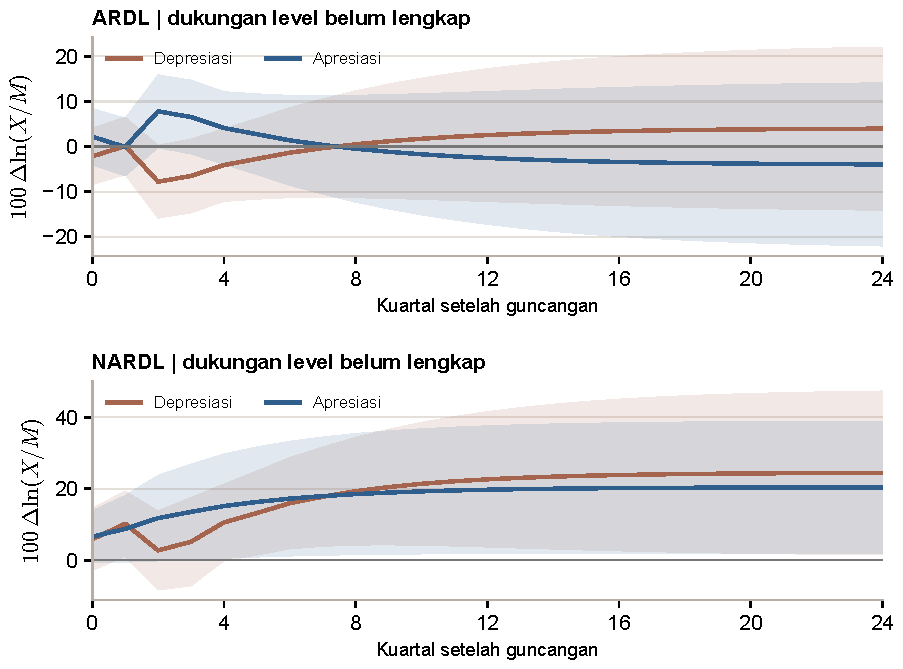
\includegraphics[width=\linewidth]{assets/response_WORLD.pdf}
\caption{Respons agregat perdagangan Indonesia. Cokelat menunjukkan depresiasi dan biru apresiasi; area berwarna adalah CI pointwise nominal 95\%. Positif berarti rasio ekspor/impor membaik. Skala vertikal dua panel berbeda.}\label{fig:world}
\end{figure}

\subsection{Apa yang dapat dipelajari dari bentuk respons}
ARDL memperlihatkan pemburukan awal pada estimasi titik sebelum perbaikan pada horizon berikutnya. Band cukup lebar, termasuk di sekitar nol pada bagian penting jalur. NARDL lebih banyak mengarah pada perbaikan, dengan fluktuasi awal yang belum menghasilkan bukti pemburukan terukur. Perbandingan ini memberi informasi mengenai bentuk yang diimplikasikan spesifikasi, tetapi tidak menggantikan syarat level yang belum terpenuhi.

Kedua arah kurs pada NARDL dapat sama-sama tampak memperbaiki rasio. Hal itu berasal dari koefisien dua partial sums yang berbeda tanda pada outcome impor/ekspor. Hasil tersebut tidak boleh langsung diperlakukan sebagai pilihan kebijakan bahwa kedua arah perubahan kurs sama-sama memberikan manfaat. Partial sums merangkum jalur historis yang berbeda, berhubungan dengan regressor lain, dan diestimasi pada sampel terbatas. Penggunaan bahasa hubungan kondisional menjadi penting ketika hasilnya tidak mendukung struktur keseimbangan yang kuat.

Baseline agregat 2010+ dipertahankan untuk pembandingan dengan run sebelumnya; perdagangan baru sendiri berasal dari workbook HS-6 pengguna. Perluasan data menjadi 2006+ tetap diestimasi dan dilaporkan dalam sensitivitas. Memilih salah satu window karena koefisiennya lebih sesuai harapan akan memperbesar risiko pencarian hasil. Kesimpulan agregat yang dapat dipertahankan adalah bahwa model utama belum memberikan hubungan jangka panjang yang kuat, bukan bahwa depresiasi terbukti tidak mempunyai pengaruh apa pun.

\subsection{Membaca arti angka tanpa mengubahnya menjadi ramalan}
Contoh yang lebih mendukung tersedia pada NARDL Indonesia--Australia. Dengan koefisien $\widehat{\beta}_-=\AusBetaMath$ dan guncangan log $-\ln(1.10)$, perubahan tampilan jangka panjang yang diimplikasikan adalah
\begin{equation}
 -100\,\widehat{\beta}_-\big[-\ln(1.10)\big]
 \simeq \AusResponseMath.
\end{equation}
Angka \AusResponse{} adalah poin log kali seratus. Perubahan persentase rasio ekspor/impor yang bersesuaian, secara aljabar, adalah
\begin{equation}
 100\left[\exp\{-\widehat{\beta}_-\delta^-\}-1\right].
\end{equation}
Pada titik estimasi itu hasilnya sekitar \AusRatioPct\%. Angka tersebut bukan peningkatan surplus dolar sebesar \AusRatioPct\%, bukan kenaikan ekspor dengan persentase yang sama, dan bukan prakiraan kebijakan tanpa syarat. Contoh ini hanya menerjemahkan satu koefisien model ke skala rasio, sambil mempertahankan seluruh asumsi dan ketidakpastian model asalnya.
